\documentclass[conference]{llncs}
% The preceding line is only needed to identify funding in the first footnote. If that is unneeded, please comment it out.
\usepackage{cite}
\usepackage{amsmath,amssymb,amsfonts}
\usepackage{algorithmic}
\usepackage{graphicx}
\usepackage{dblfloatfix}

\def\BibTeX{{\rm B\kern-.05em{\sc i\kern-.025em b}\kern-.08em
    T\kern-.1667em\lower.7ex\hbox{E}\kern-.125emX}}
\begin{document}

\title{Bayesian Learning of Finite Asymmetric Gaussian Mixtures by MH-within-Gibbs Method}

\author{Shuai Fu\inst{1} \and Nizar Bouguila\inst{2}}

\institute{Concordia University, Montreal, Canada. \textbf{Email:} \email{f\_shuai@encs.concordia.ca}
\and Concordia University, Montreal, Canada. \textbf{Email:} \email{bouguila@ciise.concordia.ca} }


\maketitle

\begin{abstract}
Asymmetric Gaussian mixture (AGM) model has been proved more exible than the classic mixture model from many aspects. In contrast with previous efforts that have been made on maximum likelihood estimation, this paper introduces a fully Bayesian learning method using Metropolis-Hastings within Gibbs sampling method to learn AGM model. We show the merits of the proposed model using synthetic data and a challenging intrusion detection applications.
\bigbreak
\textbf{Keywords - Asymmetric Gaussian Mixture, Metropolis-Hastings, Gibbs sampling, MCMC, Intrusion detection}
\end{abstract}

\section{Introduction}
Along with the development of information-based industries, network security problems are becoming more and more important today. In order to address this challenge, many data mining methodologies were proposed including both classification-based \cite{b1} and clustering-based \cite{b2} ones. However, classification-based solutions generally perform ineffectively for dynamic and variate attacking methods because changes of the intrusion patterns cannot be automatically adapted by supervised learning algorithms. Consequently, unsupervised approaches are more favorable for modern intrusion-detection.

As an efficient clustering approach, Gaussian mixtures model (GMM) \cite{b3} is widely deployed because of its outstanding suitability in several domains such as computer vision, pattern recognition and data mining. In this paper, we choose asymmetric Gaussian mixture (AGM) model \cite{b4} for modeling because it uses two variance parameters for left and right parts of each distribution in the mixture which is able to accurately model non-Gaussian datasets including asymmetric ones. 

Besides of choosing AGM model, mixture parameter learning method is also performing a critical role for clustering. The estimation of the parameters of mixture distributions can be accomplished by introducing maximum-likelihood-based expectation maximization (EM) \cite{b5} algorithm. However, EM has some drawbacks such as estimation in higher dimensions, optimization \cite{b6} and overfitting problems \cite{b7} etc,. Therefore, an alternative is the fully Bayesian approach such as Markov chain Monte Carlo (MCMC) method which has been found to be useful in many applications without given priors of parameters which can avoid overfitting problems. As a sampling-based learning method, the main difficulty of MCMC method is that, under some circumstances, direct sampling is not always straightfoward. As widely deployed implementations of MCMC method, Metropolis-Hastings (Hastings, 1970)\cite{b8} and Gibbs sampling (Geman and Geman, 1984)\cite{b9} methods can be introduced to solve this problem by applying proposal priors and posteriors and sampling one parameter by giving the others. By combining the advantages of both methods together, the Metopolis-Hastings within Gibbs method \cite{b6} is selected as the learning algorithm for AGM model.

Within the structure of this paper, Section 2 will be the illustration of AGM model and Bayesian learning processes. In Section 3, both experimental and real applications (network intrusion detection) will be tested against the AGM model and the results will be analyzed.

\section{Bayesian Model}
\subsection{Asymmetric Gaussian Mixture Model}
Assuming that the AGM model has $M$ components then the likelihood function (Elguebaly and Bouguila, 2013)\cite{b4} is defined as follows:
\begin{align}
p(\mathcal{X}|\Theta) = \prod_{i=i}^N \sum_{j=1}^Mp_jp(X_i|\xi_j)
\label{eq:1}
\end{align}
where $\mathcal{X} = (X_1,...,X_N)$ is the set of $N$ observations, $\Theta = \{p_1,...,p_M, \xi_1,...,\xi_M\}$ represents the parameter set of $M$ mixture components for the AGM model, $p_j$ (0 $< p_j \leq$ 1 and $\sum_{j=1}^Mp_j$ = 1) is the weight for each component in the mixture model and $\xi_j$ is the AGD parameters of mixture component j. Giving $X = (x_1,...,x_d)$, the probability density function (Elguebaly and Bouguila, 2013)\cite{b4} can be defined as follows:
\begin{align}
p(X|\xi_j) \propto \prod_{k=1}^{d} \frac{1}{(\sigma_{l_{jk}}+\sigma_{r_{jk}})}
\times \left\{\begin{matrix}
\exp \begin{bmatrix}
-\frac{(x_k-\mu_{jk})^2}{2(\sigma_{l_{jk}})^2}
\end{bmatrix}\ if\ x_k\ <\ \mu_{jk} \\ 
\exp \begin{bmatrix}
-\frac{(x_k-\mu_{jk})^2}{2(\sigma_{r_{jk}})^2}
\end{bmatrix}\ if\ x_k\ \geqslant\ \mu_{jk} \\ 
\end{matrix}\right.
\label{eq:2}
\end{align}
here $\xi_j = (\mu_j,\sigma_{lj},\sigma_{rj})$ is the set of parameters of component j and $\mu_j = (\mu_{j1},...,\mu_{jd})$ is the mean, $\sigma_{lj} = (\sigma_{lj1},...,\sigma_{ljd})$ and $\sigma_{rj} = (\sigma_{rj1},...,\sigma_{rjd})$ are the left and right standard deviations for AGD. To be more specific, $x_k \thicksim N(\mu_{jk},\sigma_{ljk})\ (x_k < \mu_{jk})$ and $x_k \thicksim N(\mu_{jk},\sigma_{rjk})\ (x_k \geqslant \mu_{jk})$ for each dimension.

In order to simplify the Bayesian learning process, we introduce a $M$-dimensional membership vector $Z$. For each observation $X_i, 1 < i <N, Z_i = (Z_{i1},...,Z_{iM})$ which indicates to which specific component $X_i$ belongs to (Bouguila, Ziou and Monga, 2006)\cite{b10}, such that:
\begin{align}
Z_{ij} = \left\{\begin{matrix}
1\qquad\mbox{ if }X_i\mbox{  belongs to component }j \\
0\qquad\quad\qquad \mbox{otherwise} \qquad\qquad\quad\quad \\
\end{matrix}\right.
\label{eq:3}
\end{align}
other words, $Z_{ij} = 1$ only if observation $X_i$ has the highest probability of belonging to component j and accordingly, for other components, $Z_{ij} = 0$. 

By combining the Eq. \eqref{eq:1} and Eq. \eqref{eq:3} together we derive the complete likelihood function:
\begin{align}
p(\mathcal{X}, Z|\Theta) = \prod_{i=1}^{N}\prod_{j=1}^{M}(p_jp(X_i|\xi_j))^{Z_{ij}}
\label{eq:4}
\end{align}

\subsection{Learning Algorithm}
Before describing MH-within-Gibbs learning steps, the priors and posteriors need to be clarified. Frist, we denote the postorior probability of membership vector Z as $\pi(Z|\Theta,\mathcal{X})$ (Elguebaly and Bouguila, 2011)\cite{b11}:
\begin{align}
Z^{(t)} \sim \pi(Z|\Theta^{(t-1)},\mathcal{X})
\label{eq:5}
\end{align}
then derive the number of observations belonging to a specific component j according to $Z^{(t)}$ as follows:
\begin{align}
n_j^{(t)} = \sum_{i=1}^NZ_{ij}\ (j = 1,...,M) 
\label{eq:6}
\end{align}
thus $n^{(t)}=(n_i^{(t)},...,n_M^{(t)})$ represents the number of observations belonging to each mixture component.

Since the mixture weight $p_j$ (0 $< p_j \leq$ 1 and $\sum_{j=1}^Mp_j$ = 1), a nature choice of the prior is Dirichlet distribution as follows \cite{b12}: 
\begin{align}
\pi(p_j^{(t)}) \sim \mathcal{D}(\gamma_1,...,\gamma_M )
\label{eq:7}
\end{align}
where $\gamma_j$ is known hyperparameter. Consequently, the posterior of the mixture weight $p_j$ is:
\begin{align}
p(p_j^{(t)}|Z^{(t)}) \sim \mathcal{D}(\gamma_1 + n_1^{(t)},...,\gamma_M + n_M^{(t)})
\label{eq:8}
\end{align}


Direct sampling of mixture parameters $\xi \sim p(\xi|Z,\mathcal{X})$ could be difficult so Metropolis-Hastings method should be deployed using propose proposal distributions for $\xi^{(t)} \sim q(\xi|\xi^{(t-1)})$. To be more specific, for parameters of AGM model which are $\mu$ , $\sigma_l$ and $\sigma_r$, we choose proposal distributions as follows:
\begin{align}
\mu_j^{(t)} \sim \mathcal{N}_d(\mu_j^{(t-1)},\Sigma)
\label{eq:9}
\end{align}
\begin{align}
\sigma_{lj}^{(t)} \sim \mathcal{N}_d(\sigma_{lj}^{(t-1)},\Sigma)
\label{eq:10}
\end{align}
\begin{align}
\sigma_{rj}^{(t)} \sim \mathcal{N}_d(\sigma_{rj}^{(t-1)},\Sigma)
\label{eq:11}
\end{align}
the proposal distributions are $d$-dimensional Gaussian distributions with $\Sigma$ as $d$ x $d$ identity matrix which makes the sampling as random walk MCMC process.

As the most important part of Metropolis-Hastings method, at the end of each iteration, for new generated mixture parameter set $\Theta^{(t)}$, an acceptance ratio $r$ needs to be calculated in order to make a decision whether they should be accepted or discarded for the next iteration. The acceptance ratio $r$ is given by:
\begin{align}
r = \frac{p(\mathcal{X}|\Theta^{(t)})\pi(\Theta^{(t)})q(\Theta^{(t-1)}|\Theta^{(t)})}{p(\mathcal{X}|\Theta^{(t-1)})\pi(\Theta^{(t-1)})q(\Theta^{(t)}|\Theta^{(t-1)})}
\label{eq:12}
\end{align}

where $\pi(\Theta)$ is the proposed prior distribution which can be decomposed to $d$-dimensional Gaussian distributions such that $\mu \sim \mathcal{N}_d(\eta,\Sigma)$ and $\sigma_l, \sigma_r \sim \mathcal{N}_d(\tau,\Sigma)$ given known hyperparameters $\eta$ and $\tau$. Since mixture weight $p$ has been computed previously during the Gibbs sampling part, it should not be included in Eq. \eqref{eq:12}. Further information about the calculation of acceptance ratio $r$ is explained in Appendix A.

Once acceptance ratio $r$ is derived by Eq. \eqref{eq:15}, compute acceptance probability $\alpha = min[1,r]$ \cite{b13}. Then $u \sim U_{[0,1]}$ is supposed to be generated randomly. If $\alpha < u$, the proposed move should be accepted and parameters should be updated by $p^{(t)}$ and $\xi^{(t)}$ for next iteration. Otherwise, discard $p^{(t)}$, $\xi^{(t)}$ and set $p^{(t)} = p^{(t-1)}$, $\xi^{(t)} = \xi^{(t-1)}$.

We summarize the MH-within-Gibbs learning process for AGM model as the following steps:
\bigbreak
\noindent\textbf{Input:} Data observations $\mathcal{X}$ and component number $M$ \\
\textbf{Output:} AGM mixture parameter set $\Theta$
\bigbreak

\begin{enumerate}
\item Initialization
\item Step $t$: For $t = 1,\ldots$
\begin{enumerate}
\item[]\textbf{Gibbs sampling part}
\item Generate $Z^{(t)}$ from Eq. \eqref{eq:5}
\item Compute $n_j^{(t)}$ from Eq. \eqref{eq:6}
\item Generate $p_j^{(t)}$ from Eq. \eqref{eq:8}
\item[] \textbf{Metropolis-Hastings part}
\item Sample $\xi_j^{(t)}$ ($\mu_j^{(t)}, \sigma_{lj}^{(t)}, \sigma_{rj}^{(t)}$) from Eqs. \eqref{eq:9} \eqref{eq:10} \eqref{eq:11}
\item Compute acceptance ratio $r$ from Eq. \eqref{eq:15}
\item Generate $\alpha = min[1,r]$ and $u \sim U_{[0,1]}$
\item If $\alpha \geq u$ then $\xi^{(t)} = \xi^{(t-1)}$
\end{enumerate}
\end{enumerate}


\section{Experimental Results}
\subsection{Design of Experiments}
We apply the AGM model to both synthetic data and intrusion detection application. For synthetic data validation part, testing observations will be generated from AGD with known component number $M$. NSL-KDD dataset \cite{b14} is selected for intrusion detection part.

\subsection{Synthetic Data}
The main goals of this section are feasibility analysis and efficiency evaluation of the AGM learning algorithm.

Observation number is set to 300 spliting into two groups ($M$ = 2). Hyperparameters are set accordingly that $\gamma_j = 1$ \cite{b15} for sampling mixture weight $p_j$ from Eq. \eqref{eq:8}. $\eta$ and $\tau$ are $d$-dimensional zero vectors in prior distributions of mixture parameter set $\xi$.

Different proposed component numbers ($M' = 1,\dots,5$) are applied during the AGM learning process and the statistics are summarized in Table \ref{tab1}. In order to distinguish the best value of the proposed component number $M'$, we introduce marginal likelihood \cite{b6} as a measurement that the best fit $M'$ should have the maximum marginal likelihood value. Obviously, the best result is derived when proposed component number $M'$ equals to original component number $M$ ($M' = M = 2$) which is shown as Fig. \ref{fig:1}. The probability density diagrams is plotted for both original and estimated AGM components and the polylines show the trace of accepted moves for each component.

Then we focus on the best fit result , the accuracy is evaluated by calculating the Euclidean distance between original and estimated mixture parameter sets $\xi$ and $\hat{\xi}$ (Table \ref{tab2}). In summary, the estimation of mean is accurate because the Euclidean distance between $\mu_j$ and $\hat{\mu}_j$ are small but the distance between standard deviation $\sigma_{lj}, \sigma_{rj}$ and $\hat{\sigma}_{lj}, \hat{\sigma}_{rj}$ are significant. Since membership vector $Z$ is involved for hard-clustering so this difference will not affect the clustering result too much.

 
\begin{table}[h]
\caption{AGM Learning Statistics ($M = 2,\ M' = 1,\dots,5,\ iterations = 300$)}
\begin{center}
\begin{tabular}{|c|c|c|c|}
\hline
\multicolumn{1}{|p{2cm}|}{\centering \textbf{Component Number $M'$}} & \multicolumn{1}{|p{2cm}|}{\centering \textbf{\textit{Moves Accepted}}} & \multicolumn{1}{|p{2cm}|}{\centering \textbf{\textit{Acceptance Ratio}}} & \textbf{\textit{ML$^{\mathrm{a}}$}}\\
\hline
1 & 22 & 7.33\% & -1596.143  \\
2 & 11 & 3.67\% & -1500.370 \\
3 & 14 & 4.67\% & -1684.518 \\
4 & 63 & 21.00\% & -1522.148 \\
5 & 39 & 13.00\% & -1517.533 \\
\hline
\multicolumn{4}{l}{$^{\mathrm{a}}$Marginal likelihood.}
\end{tabular}
\label{tab1}
\end{center}
\end{table}

\begin{figure}
\centering
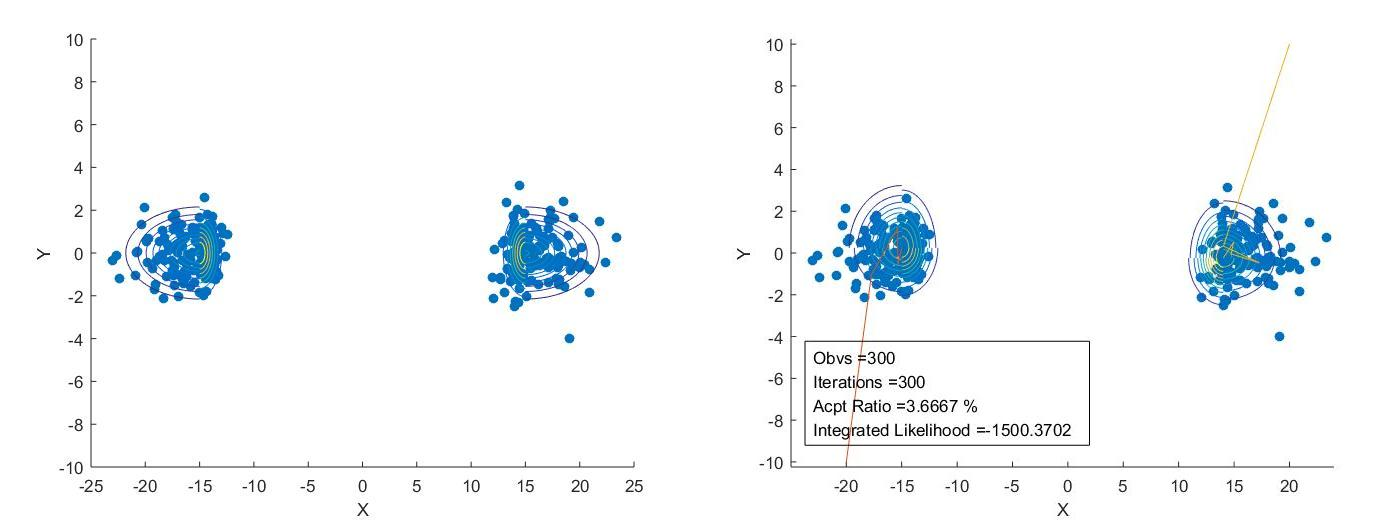
\includegraphics[width=0.6\paperwidth ]{02.jpg}
\caption{Original synthetic observations and learning result ($M' = M = 2$)}
\label{fig:1}
\end{figure}

\begin{table}[h]
\caption{Accuracy Analysis ($M' = M = 2$)}
\begin{center}
\begin{tabular}{|c|c|c|c|}
\hline
\multicolumn{1}{|p{3cm}|}{\centering \textbf{Component Number $j = 1$}} & \multicolumn{1}{|p{2cm}|}{\centering \textbf{Mean \\($\mu_j$)}} & \multicolumn{1}{|p{3cm}|}{\centering \textbf{Left Standard deviation ($\sigma_{lj}$)}} & \multicolumn{1}{|p{3cm}|}{\centering \textbf{Right Standard deviation ($\sigma_{rj}$)}}\\
\hline
$\xi$ & [-15.00, 0.00] & [10.00, 1.00] & [1.00, 1.00]  \\
$\hat{\xi}$ & [-14.99, 0.25] & [4.77, 1.13] & [2.31, 1.88] \\
Euclidean Distance & 0.246 & 5.236 & 1.581 \\
\hline
\multicolumn{1}{|p{3cm}|}{\centering \textbf{Component Number $j = 2$}} & \multicolumn{1}{|p{2cm}|}{\centering \textbf{Mean \\($\mu_j$)}} & \multicolumn{1}{|p{3cm}|}{\centering \textbf{Left Standard deviation ($\sigma_{lj}$)}} & \multicolumn{1}{|p{3cm}|}{\centering \textbf{Right Standard deviation ($\sigma_{rj}$)}}\\
\hline
$\xi$ & [15.00, 0.00] & [1.00, 1.00] & [10.00, 1.00]  \\
$\hat{\xi}$ & [14.02, -0.24] & [2.04, 1.04] & [5.70, 1.59] \\
Euclidean Distance & 1.010 & 1.036 & 4.338 \\
\hline
\end{tabular}
\label{tab2}
\end{center}
\end{table}




\subsection{Intrusion Detection (TBD)}
TBD

\section{Conclusion (TBD)}
TBD

\section*{Acknowledgment (TBD)}
TBD

\section*{Appendix A}
\subsection{Derivation of Acceptance Ratio $r$ by Eq. \eqref{eq:12}}
The derivation of acceptance ratio $r$ is based on the assumption that mixture parameters are independent from each other which means that:
\begin{multline}
\qquad\qquad\pi(\Theta) = \pi(p,\xi) = \pi(\xi) \\
= \prod_{j=1}^M\pi(\mu_j)\pi(\sigma_{lj})\pi(\sigma_{rj}) \qquad\qquad\qquad\qquad\qquad\\
= \prod_{j=1}^M\mathcal{N}_d(\mu_j|\eta,\Sigma)\mathcal{N}_d(\sigma_{lj}|\tau,\Sigma)\mathcal{N}_d(\sigma_{rj}|\tau,\Sigma)\qquad\qquad\qquad
\label{eq:13}
\end{multline}
in Eq. \eqref{eq:14}, since the mixture weigh $p$ is generated following Gibbs sampling method which acceptance ratio is always 1, it should be excluded from Metropolis-Hastings estimation step. Accordingly, apply the same rule to the proposal distribution as well:
\begin{multline}
\qquad\qquad q(\Theta^{(t)}|\Theta^{(t-1)}) = q(\xi^{(t)}|\xi^{(t-1)}) \\
= \prod_{j=1}^M\mathcal{N}_d(\mu_j^{(t)}|\mu_j^{(t-1)},\Sigma)\mathcal{N}_d(\sigma_{lj}^{(t)}|\sigma_{lj}^{(t-1)},\Sigma)\mathcal{N}_d(\sigma_{rj}^{(t)}|\sigma_{rj}^{(t-1)},\Sigma)
\label{eq:14}
\end{multline}
by combining Eqs. \eqref{eq:2} \eqref{eq:4} \eqref{eq:9} \eqref{eq:10} \eqref{eq:11} \eqref{eq:14} and \eqref{eq:15}, equation \eqref{eq:12} can be written as follows:

\begin{multline}
\qquad\qquad r = \frac{p(\mathcal{X}|\Theta^{(t)})\pi(\Theta^{(t)})q(\Theta^{(t-1)}|\Theta^{(t)})}{p(\mathcal{X}|\Theta^{(t-1)})\pi(\Theta^{(t-1)})q(\Theta^{(t)}|\Theta^{(t-1)})} \\
= \prod_{i=i}^N \prod_{j=1}^M(\frac{p(X_i|\mu_j^{(t)},\sigma_{lj}^{(t)},\sigma_{rj}^{(t)})}
{p(X_i|\mu_j^{(t-1)},\sigma_{lj}^{(t-1)},\sigma_{rj}^{(t-1)})} \qquad\qquad\\
\times \frac{\mathcal{N}_d(\mu_j^{(t)}|\eta,\Sigma)\mathcal{N}_d(\sigma_{lj}^{(t)}|\tau,\Sigma)\mathcal{N}_d(\sigma_{rj}^{(t)}|\tau,\Sigma)}{\mathcal{N}_d(\mu_j^{(t-1)}|\eta,\Sigma)\mathcal{N}_d(\sigma_{lj}^{(t-1)}|\tau,\Sigma)\mathcal{N}_d(\sigma_{rj}^{(t-1)}|\tau,\Sigma)} \\
\times \frac{\mathcal{N}_d(\mu_j^{(t-1)}|\mu_j^{(t)},\Sigma)\mathcal{N}_d(\sigma_{lj}^{(t-1)}|\sigma_{lj}^{(t)},\Sigma)\mathcal{N}_d(\sigma_{rj}^{(t-1)}|\sigma_{rj}^{(t)},\Sigma)}{\mathcal{N}_d(\mu_j^{(t)}|\mu_j^{(t-1)},\Sigma)\mathcal{N}_d(\sigma_{lj}^{(t)}|\sigma_{lj}^{(t-1)},\Sigma)\mathcal{N}_d(\sigma_{rj}^{(t)}|\sigma_{rj}^{(t-1)},\Sigma)}
\label{eq:15}
\end{multline}

\begin{thebibliography}{[MT1]}
\bibitem{b1} Puttini, R.S., Marrakchi, Z. and Mé, L., 2003, March. A Bayesian Classification Model for Real‐Time Intrusion Detection. In AIP Conference Proceedings (Vol. 659, No. 1, pp. 150-162). AIP.

\bibitem{b2} Zhong, S., Khoshgoftaar, T.M. and Seliya, N., 2007. Clustering-based network intrusion detection. International Journal of reliability, Quality and safety Engineering, 14(02), pp.169-187.

\bibitem{b3} Rasmussen, C.E., 2000. The infinite Gaussian mixture model. In Advances in neural information processing systems (pp. 554-560).

% \bibitem{b4} Bouguila, N. (2008). Finite general Gaussian mixture modeling and application to image and video foreground segmentation. Journal of Electronic Imaging, 17(1), p.013005.

\bibitem{b4} Elguebaly, T. and Bouguila, N. (2013). Background subtraction using finite mixtures of asymmetric Gaussian distributions and shadow detection. Machine Vision and Applications, 25(5), pp.1145-1162.

\bibitem{b5} Dempster, A.P., Laird, N.M. and Rubin, D.B., 1977. Maximum likelihood from incomplete data via the EM algorithm. Journal of the royal statistical society. Series B (methodological), pp.1-38.

\bibitem{b6} Bouguila, N., Ziou, D. and Hammoud, R. (2008). On Bayesian analysis of a finite generalized Dirichlet mixture via a Metropolis-within-Gibbs sampling. Pattern Analysis and Applications, 12(2), pp.151-166.

\bibitem{b7} Bouguila, N. and Elguebaly, T. (2012). A fully Bayesian model based on reversible jump MCMC and finite Beta mixtures for clustering. Expert Systems with Applications, 39(5), pp.5946-5959.

\bibitem{b8} Hastings, W. (1970). Monte Carlo Sampling Methods Using Markov Chains and Their Applications. Biometrika, 57(1), p.97.

\bibitem{b9} Geman, S. and Geman, D. (1984). Stochastic Relaxation, Gibbs Distributions, and the Bayesian Restoration of Images. IEEE Transactions on Pattern Analysis and Machine Intelligence, PAMI-6(6), pp.721-741.

\bibitem{b10} Bouguila, N., Ziou, D. and Monga, E. (2006). Practical Bayesian estimation of a finite beta mixture through gibbs sampling and its applications. Statistics and Computing, 16(2), pp.215-225.

\bibitem{b11} Elguebaly, T. and Bouguila, N. (2011). Bayesian learning of finite generalized Gaussian mixture models on images. Signal Processing, 91(4), pp.801-820.

\bibitem{b12} Marin, J.M. and Mengersen, K.R.C., 2005. Handbook of Statistics: Bayesian modelling and inference on mixtures of distributions, Vol. 25.

\bibitem{b13} Luengo, D. and Martino, L., 2013, May. Fully adaptive gaussian mixture metropolis-hastings algorithm. In Acoustics, Speech and Signal Processing (ICASSP), 2013 IEEE International Conference on (pp. 6148-6152). IEEE.

\bibitem{b14} Tavallaee, M., Bagheri, E., Lu, W. and Ghorbani, A.A., 2009, July. A detailed analysis of the KDD CUP 99 data set. In Computational Intelligence for Security and Defense Applications, 2009. CISDA 2009. IEEE Symposium on (pp. 1-6). IEEE.
Vancouver	

\bibitem{b15} Stephens, M., 2000. Bayesian analysis of mixture models with an unknown number of components-an alternative to reversible jump methods. Annals of statistics, pp.40-74.

\end{thebibliography}
\end{document}
